\input{preamble.tex}
\usepackage{eurosym}

\newcommand{\C}{\mathcal{C}}
\begin{document}
\pagestyle{fancy}
\fancyhead[L]{Seconde}
\fancyhead[C]{\textbf{Evaluation flash - récap semestre 1}}
\fancyhead[R]{\today}

\reversemarginpar

\null\vspace{-30pt}
Nom / Prénom : \\

Consignes particulières : 
\begin{itemize}[label=$\bullet$]
	\item 
	La calculatrice est \textbf{interdite}.
	\item 
	Le devoir peut être fait entièrement sur cette feuille.
	\item 
	Toute trace de recherche est prise en compte.
	%\item 
	%L'abbréviation $\tq$ signifie ``tel que''.
\end{itemize}

\hrule

\exe{2}{
Résoudre dans $\R$ l'équation $\dfrac54 x - 8 = \dfrac13$ 
\vspace{5cm}
}{exe:1}{

}

\exe{2}{
Représenter, dans le repère ci-dessous, une partie de la courbe repésentative de la fonction :
\[ \begin{array}{c c c c}
f : & \R & \to & \R \\
& x & \mapsto & \dfrac13 x + 2
\end{array} \]
\begin{center}
	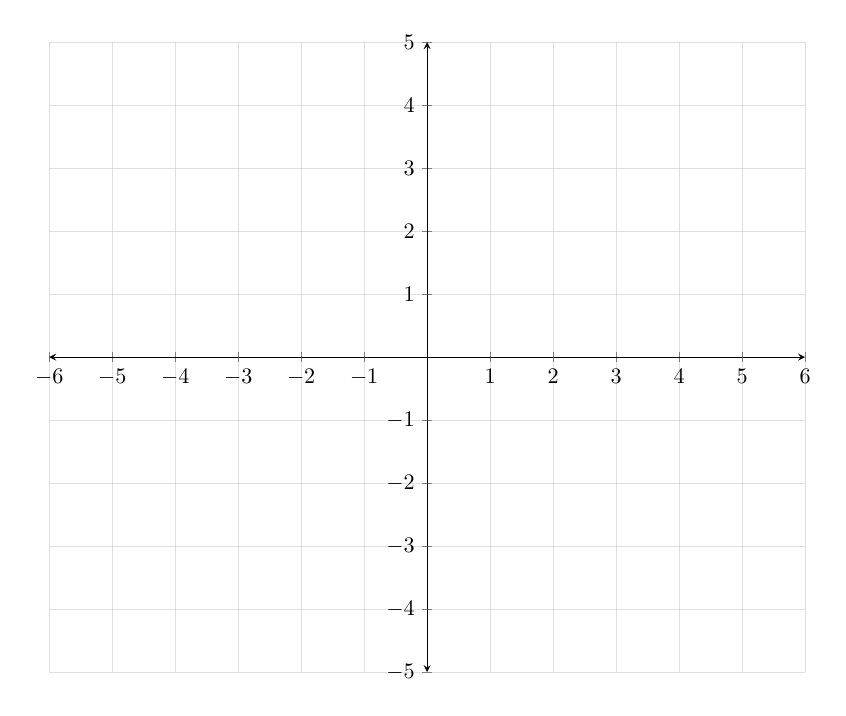
\begin{tikzpicture}[>=stealth, scale=.8]
		\begin{axis}[xmin = -6, xmax=6, ymin=-5, ymax=5, axis x line=middle, axis y line=middle, axis line style=<->, xlabel={}, ylabel={}, grid=both, grid style = {opacity=.5}, clip=false, xtick distance = 1, ytick distance=1, x=1cm, y=1cm]
		\end{axis}
	\end{tikzpicture}
\end{center}
Déterminer graphiquement l'antécédent de $y=2$ par $f$.
}{exe:2}{

}

\newpage

\exe{2}{
Le prix d'un article subit deux diminutions successives de $20 \%$. 
Quel est son prix final s'il coûtait, initialement, 50 \euro~?
\vspace{5cm}
}{exe:3}{

}

\exe{2}{
Calculer la distance entre les points $A(5 ; 1)$ et $B(1; -2)$. 
\vspace{3cm}
\newline
Les placer dans le repère ci-dessous 
\begin{center}
	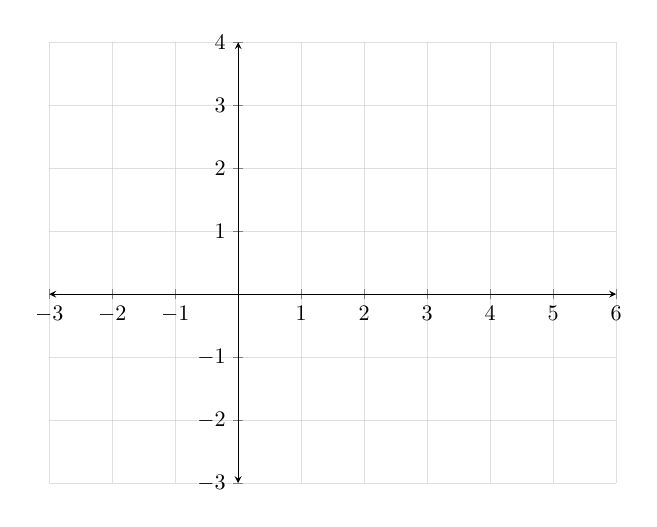
\begin{tikzpicture}[>=stealth, scale=.8]
		\begin{axis}[xmin = -3, xmax=6, ymin=-3, ymax=4, axis x line=middle, axis y line=middle, axis line style=<->, xlabel={}, ylabel={}, grid=both, grid style = {opacity=.5}, clip=false, xtick distance = 1, ytick distance=1, x=1cm, y=1cm]
		\end{axis}
	\end{tikzpicture}
\end{center}
}{exe:4}{

}

\exe{2}{
Calculer 
\begin{enumerate}[label=(\alph*)]
\item Donner un nnombre rationnel \textbf{non décimal}
\vspace{3cm}
\item Encadrer le nombre $\frac13$ à $10^{-3}$ près.
\vspace{3cm}
\end{enumerate}
}{exe:5}{

}


%%%%%%%%%%%%

\newpage
\fancyhead[C]{\textbf{Solutions}}
\shipoutAnswer

\end{document}
 